\documentclass[12pt,a4paper]{article}
\usepackage{ctex} % 支持中文
\usepackage{graphicx}
\usepackage{geometry}
\usepackage{array}
\usepackage{setspace}
\usepackage{xeCJK}
\usepackage{indentfirst} % 首行缩进
\usepackage{amsmath}
\usepackage{amsthm}
\usepackage{float} % 用于图片浮动控制 H 选项
\usepackage{subfigure} % 支持子图
\usepackage{booktabs} % 提供更美观的表格线
\usepackage{multirow} % 支持表格单元格合并
\usepackage{caption} % 自定义图表标题

% 设置页边距
\geometry{left=2.5cm,right=2.5cm,top=2.5cm,bottom=2.5cm}

% 设置默认字体为宋体小四, 可根据需要调整
\setCJKmainfont[BoldFont=SimHei]{SimSun}
\zihao{-4}

% 取消首行缩进 (根据用户最新文档保留)
\setlength{\parindent}{0em}

% 定义一些数学符号的快捷方式 (如果需要)
\newcommand{\rmcm}{\mathrm{\,cm}}
\newcommand{\rmmm}{\mathrm{\,mm}}

\begin{document}

% 页眉部分
\begin{center}
  \begin{tabular}{p{0.3\textwidth}p{0.7\textwidth}}
    
\includegraphics[width=0.3\textwidth]{assets/scut_logo.png} & % 学校Logo，请确保路径正确
    \zihao{3}\songti\textbf{大学物理实验（一）实验报告}
  \end{tabular}
\end{center}

% 标题
\begin{center}
  {\zihao{-3}\songti\textbf{薄透镜焦距的测量}}
\end{center}

\vspace{0.8cm}

% 学生信息表格
\noindent \begin{tabular}{@{}llll}
24级\underline{\makebox[3cm][c]{x}} 班 & 
姓名\underline{\makebox[3cm][c]{Pinco Li}} & 
小组序号\underline{\makebox[3cm][c]{x}} \\[2ex]
\end{tabular}

\noindent \begin{tabular}{@{}llll}
实验日期 2025 年\underline{\makebox[1cm][c]{5}} 月 \underline{\makebox[1cm][c]{16}} 日 
& 第 12 周 
& 星期\underline{\makebox[2cm][c]{五}} 
& 指导老师\underline{\makebox[2cm][c]{x}} \\[2ex]
\end{tabular}

\noindent 同组同学\underline{\makebox[5cm][c]{x}}

\vspace{0.5cm}
\noindent\textbf{一、实验目的}

\begin{enumerate}
    \item 深化对薄透镜成像原理的理解
    \item 通过实践学习操作平行光聚焦法测凸透镜焦距
    \item 通过实践学习操作二次成像法（共轭法）测凸透镜焦距
    \item 通过实践学习操作自准直法测量凸透镜焦距
    \item 通过实践学习操作二次成像法测量凹透镜焦距
    \item 提升实验设计与数据分析能力
\end{enumerate}

\vspace{0.5cm}
\noindent\textbf{二、实验仪器}

\begin{enumerate}
    \item 光具座导轨 (附毫米刻度，最小分度 $1\rmmm$)
    \item 凸透镜 $L_1$ (编号“1”, 焦距约 $7 \rmcm$)
    \item 凸透镜 $L_2$ (编号“2”, 焦距约 $20 \rmcm$)
    \item 凸透镜 $L_3$ (编号“3”, 焦距约 $25 \rmcm$)
    \item 凹透镜 (无编号，未知焦距)
    \item 平行白光源
    \item 溴钨灯
    \item 物屏
    \item 像屏 (白屏)
    \item 平面反射镜
\end{enumerate}
    \begin{figure}[H]
        \centering
        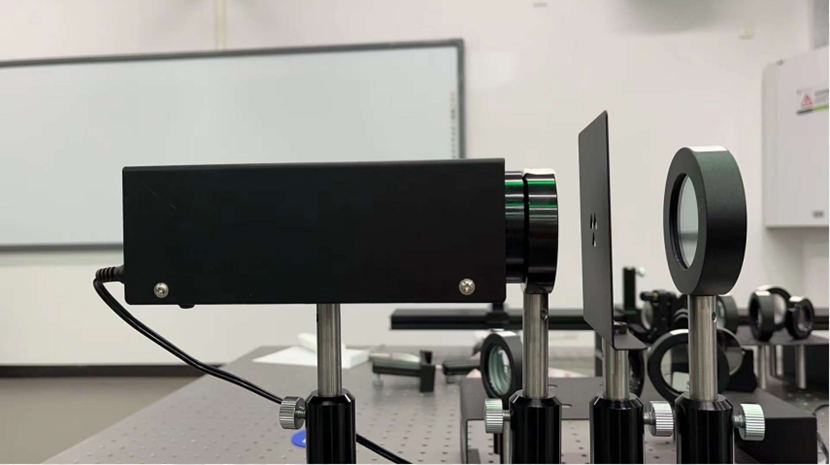
\includegraphics[clip,scale=0.7,trim={0 50 0 30}]{assets/fig1.png}
        \caption{平行白光源示意图}
        \label{fig:parallel_light_source_detailed_refined}
    \end{figure}
    \begin{figure}[H]
        \begin{minipage}[t]{0.48\linewidth}
            \centering
            
\includegraphics[clip,scale=0.6,trim={0 0 0 0}]{assets/fig2.png}
            \caption{透镜示意图}
            \label{fig:lenses_detailed_refined}
        \end{minipage}
        \hfill
        \begin{minipage}[t]{0.48\linewidth}
            \centering
            
\includegraphics[clip,scale=0.45]{assets/fig3.png}
            \caption{物屏示意图}
            \label{fig:object_screen_detailed_refined}
        \end{minipage}
    \end{figure}
    \begin{figure}[H]
        \centering
        
\includegraphics[clip,scale=0.8,trim={0 30 0 0}]{assets/fig4.png}
        \caption{光具座上光学元件放置示意图}
        \label{fig:optical_setup_detailed_refined}
    \end{figure}

\vspace{0.5cm}
\noindent\textbf{三、实验原理}

薄透镜是指中心厚度远小于其球面曲率半径的透镜。在近轴条件下，薄透镜的物距 $u$、像距 $v$ 与焦距 $f$ 遵循高斯成像公式：$\frac{1}{v} + \frac{1}{u} = \frac{1}{f}$。符号约定：实物实像时 $u, v$ 为正；虚物虚像时为负（本实验中凹透镜虚物 $u$ 取负）。凸透镜焦距 $f$ 为正，凹透镜 $f$ 为负。

\noindent\textbf{1. 凸透镜焦距的测量方法}

\noindent\textit{(1) 平行光聚焦法：}平行于主轴的光线经凸透镜会聚于焦点，透镜光心到焦点的距离即为焦距。
\begin{figure}[H]
    \centering
    
\includegraphics[clip,scale=0.8,trim={0 0 0 0}]{assets/fig5.png}
    \caption{平行光聚焦法测量凸透镜焦距示意图}
    \label{fig:parallel_focusing_main_detailed_refined}
\end{figure}

\noindent\textit{(2) 二次成像法（共轭法）：}固定物屏与像屏距离 $L > 4f$，移动透镜可在屏上获得两次清晰实像。设两次成像透镜移动距离为 $d$，则焦距 $f = \frac{L^2 - d^2}{4L}$。
\begin{figure}[H]
    \centering
    
\includegraphics[clip,scale=0.8,trim={0 0 0 0}]{assets/fig8.png}
    \caption{二次成像法测量凸透镜焦距示意图}
    \label{fig:secondary_imaging_main_detailed_refined}
\end{figure}

\noindent\textit{(3) 自准直法：}物位于凸透镜焦平面上时，经透镜折射成平行光，被垂直于光轴的平面镜反射后，再次通过透镜会聚于焦平面，在物屏上形成与原物等大、倒立的实像。此时物屏到透镜光心的距离即为焦距。
\begin{figure}[H]
    \centering
    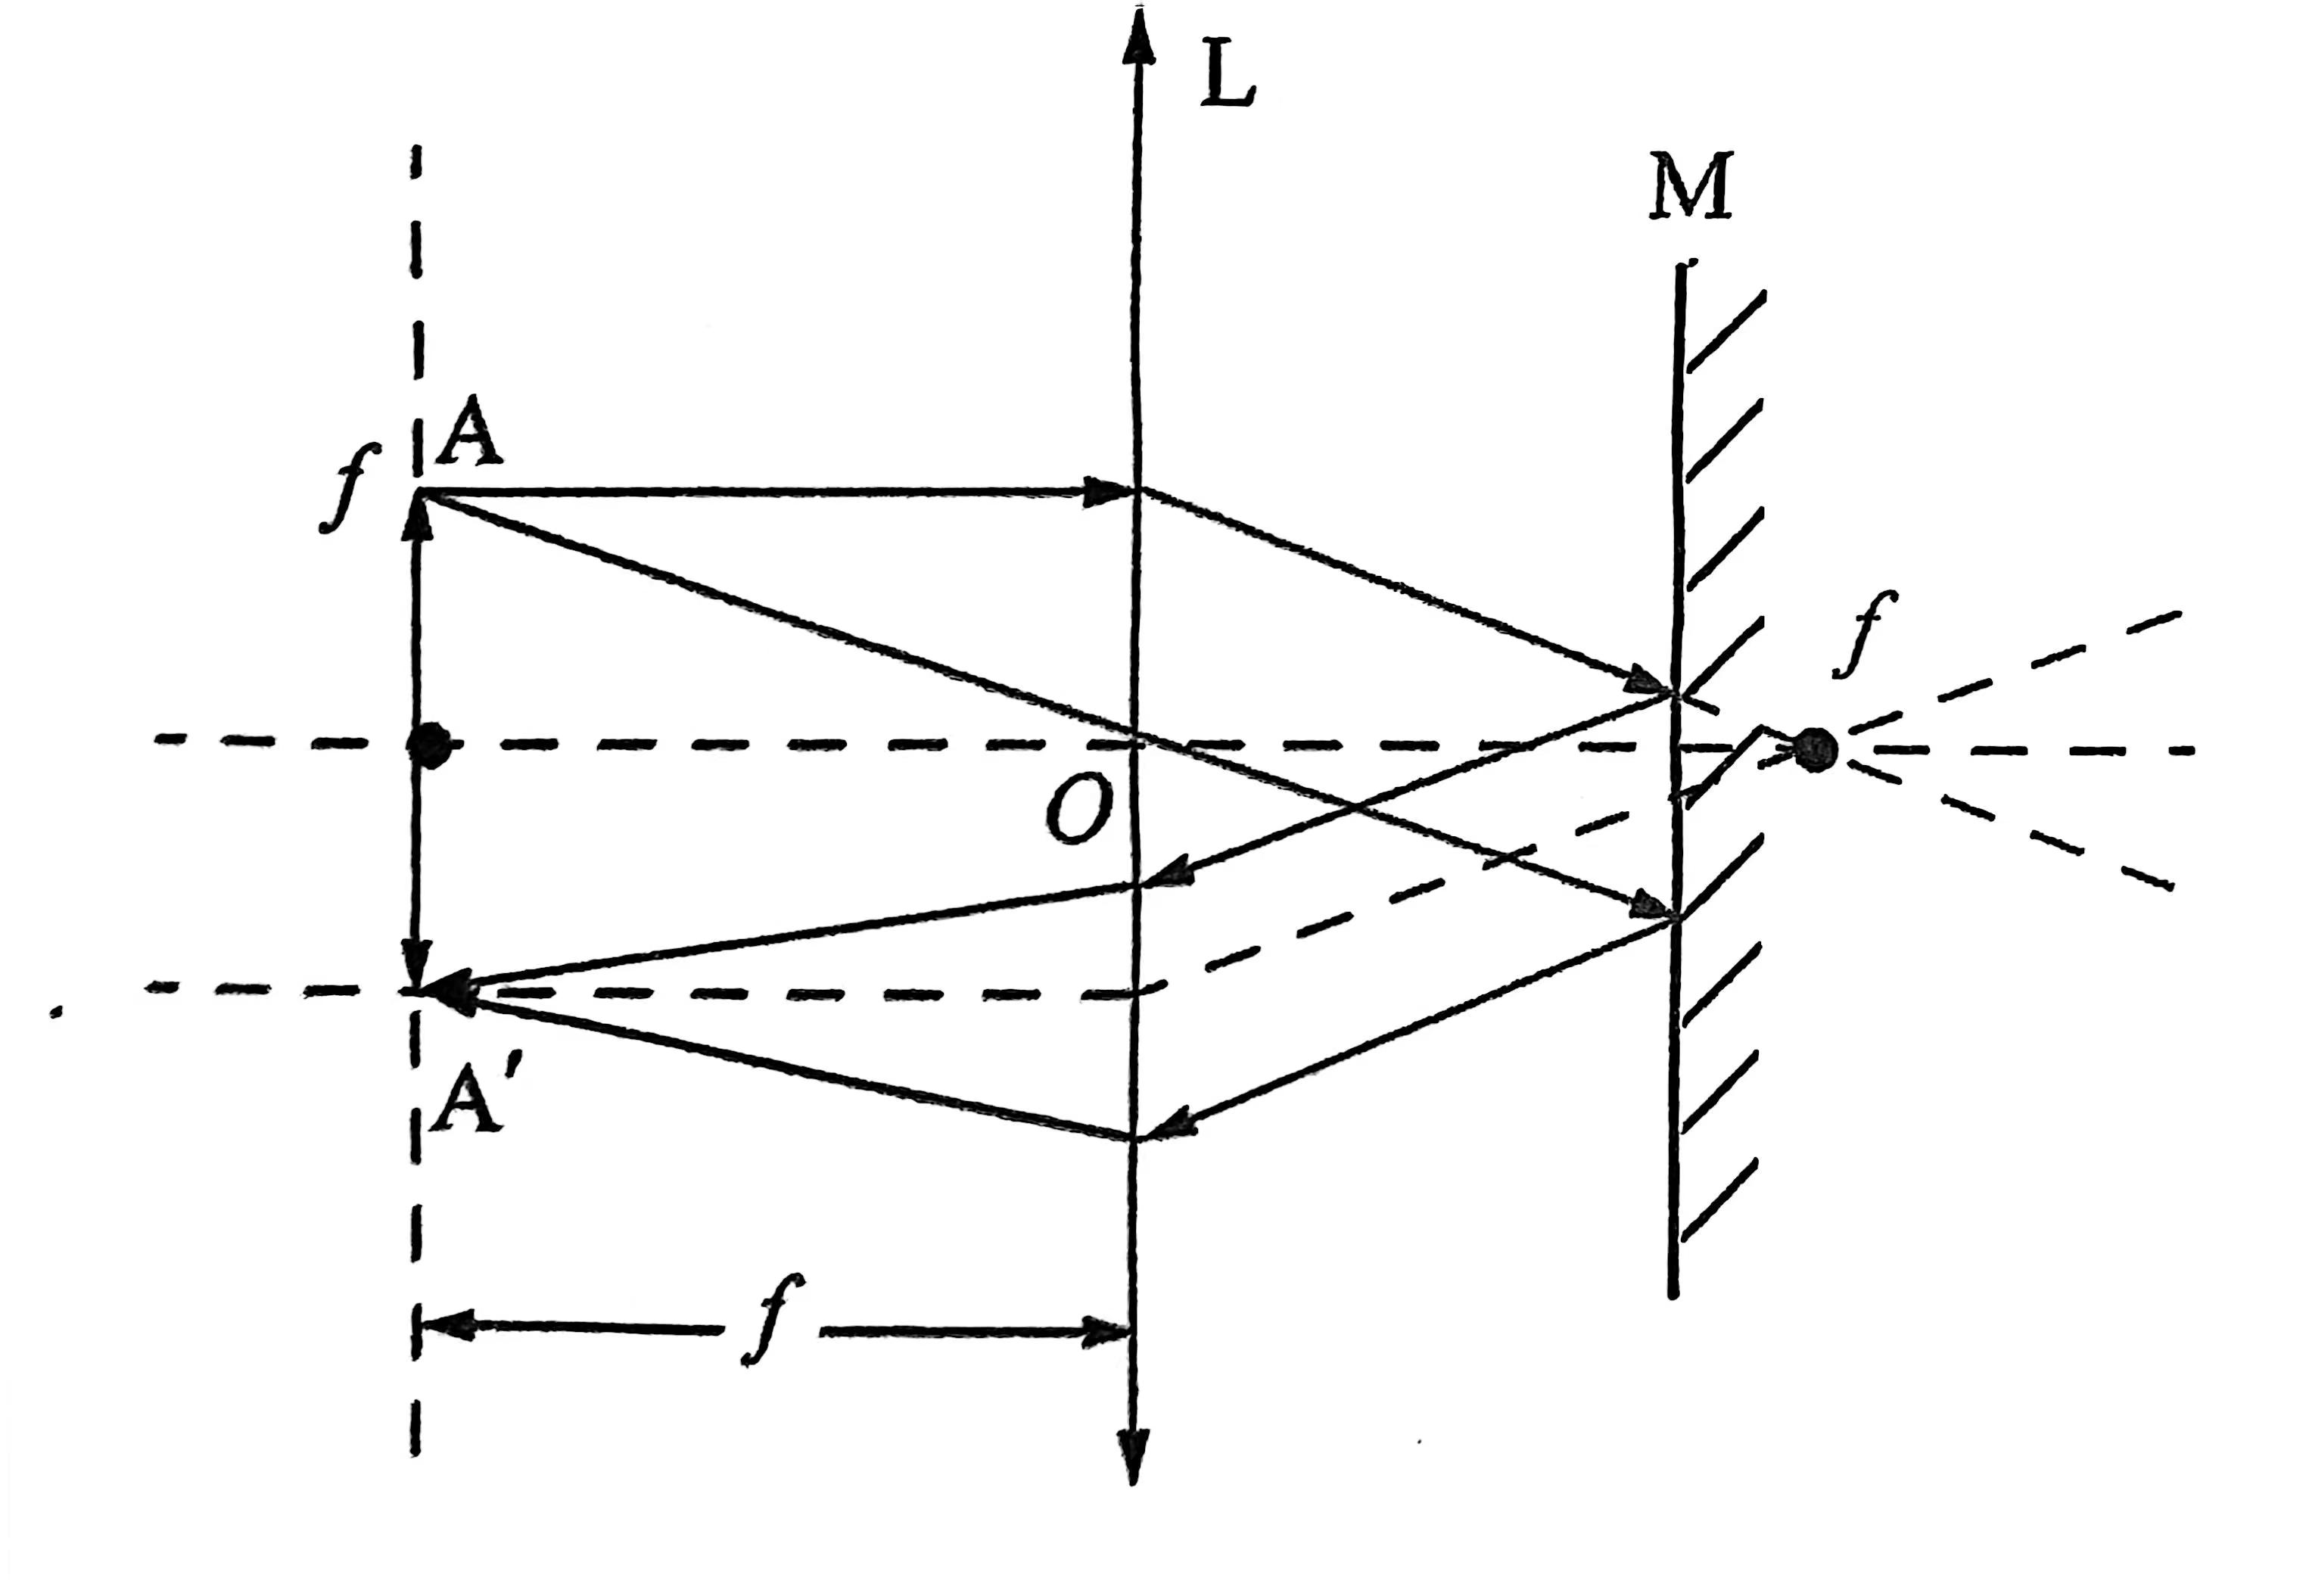
\includegraphics[width=0.7\textwidth]{assets/zizhunfig.jpg}
    \caption{自准直法测量凸透镜焦距光路示意图 (概念图)}
    \label{fig:self_collimation_main_detailed_refined}
\end{figure}
        
\noindent\textbf{2. 凹透镜焦距的测量方法}
采用二次成像法（辅助透镜法）：先用辅助凸透镜 $L_A$ 对物成实像 $A'$ (位置 $x_{A1}$)。在 $L_A$ 与 $A'$ 间放入待测凹透镜 $L_2$ (位置 $x_{L2}$)，$A'$ 作为 $L_2$ 的虚物，物距 $u = x_{A1} - x_{L2}$ (取负值)。调整最终像屏得到实像 $A''$ (位置 $x_{A2}$)，像距 $v = x_{A2} - x_{L2}$ (取正值，若像在凹透镜右侧)。代入公式计算 $f$。
\begin{figure}[H]
    \centering
    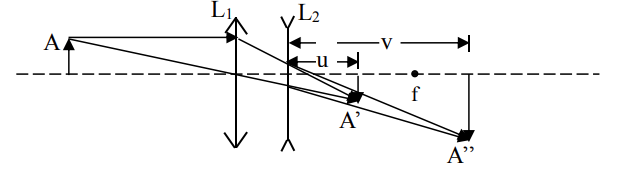
\includegraphics[clip,scale=0.8,trim={0 0 0 0}]{assets/fig9.png}
    \caption{二次成像法测量凹透镜焦距示意图}
    \label{fig:concave_lens_measurement_main_detailed_refined}
\end{figure}

\vspace{0.5cm}
\noindent\textbf{四、实验内容与步骤}

\noindent\textbf{1. 光学元件的共轴调节}
粗调各元件中心大致等高共轴。细调采用“等高法”或“小像追大像法”：在 $L > 4f$ 条件下，观察放大像与缩小像中心是否重合，调节物屏或透镜高度及横向位置，直至两像中心完全重合。
\begin{figure}[H]
    \centering
    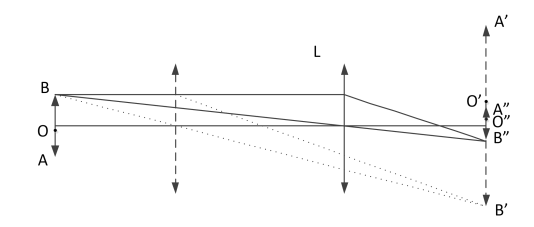
\includegraphics[clip,scale=0.8,trim={0 0 0 0}]{assets/fig10.png}
    \caption{共轴调节示意图}
    \label{fig:coaxial_adjustment_main_detailed_refined}
\end{figure}

\noindent\textbf{2. 测量凸透镜焦距}

\noindent\textit{(1) 平行光直接测量凸透镜 $L_1$、$L_2$、$L_3$ 焦距：} 将平行光源、待测凸透镜、像屏共轴放置。移动像屏至获得最清晰、最小光点，测量透镜到像屏距离即为焦距。分别测量 $L_1$、$L_2$、$L_3$。

\noindent\textit{(2) 二次成像法测量凸透镜 $L_1$ 焦距：} 固定物屏与像屏距离 $L$ ($L > 4f_{\text{$L_1$}}$)。移动 $L_1$ 找到两个清晰成像位置 $X_1, X_2$，记录并计算。重复两次。

\noindent\textit{(3) 自准直法测量凸透镜 $L_1$ 焦距：} 将光源、物屏、$L_1$、平面镜共轴放置，平面镜垂直光轴。调整 $L_1$ 或物屏位置，使物屏上得到与原物等大、倒立、清晰重合的像，记录物屏到 $L_1$ 距离。重复两次。

\noindent\textbf{3. 二次成像法测量凹透镜焦距}
先用辅助凸透镜 $L_A$ 成实像 $A'$ 于 $x_{A1}$。在 $L_A$ 与 $A'$ 间放入凹透镜 $L_2$ 于 $x_{L2}$。调整最终像屏在 $x_{A2}$ 处得清晰实像 $A''$。记录 $x_{A1}, x_{L2}, x_{A2}$ 并计算。重复两次。
\begin{figure}[H]
    \centering
    \includegraphics[clip,scale=0.07,trim={0 400 0 900}]{assets/fig14.jpg}
    \caption{测量凹透镜焦距的实验装置示意图}
    \label{fig:concave_lens_setup_photo_main_detailed_refined}
\end{figure}

\noindent\textbf{4. 光学仪器的组装与观察 (选做)}
选用合适的透镜（$L_1$、$L_2$、$L_3$）组装显微镜和望远镜，观察其成像特点。记录各透镜的焦距、位置以及中间像的位置。

\vspace{0.5cm}
\noindent\textbf{五、实验数据记录与处理}

\noindent\textbf{1. 凸透镜焦距测量}

\noindent\textit{(1) 表1：平行光直接测量凸透镜 $L_1$、$L_2$、$L_3$ 焦距}
\begin{table}[H]
    \centering
    \caption{平行光直接测量凸透镜焦距数据}
    \begin{tabular}{cc}
        \toprule[1.5pt]
        凸透镜编号 & 焦距 $f~(\rmcm)$ \\
        \midrule
        $L_1$ (镜1)   & 7.02            \\
        $L_2$ (镜2)   & 19.95           \\
        $L_3$ (镜3)   & 25.05           \\
        \bottomrule[1.5pt]
    \end{tabular}
    \label{tab:convex_direct_scan}
\end{table}

\noindent\textit{(2) 表2：二次成像法（共轭法）测量凸透镜 $L_1$ 焦距}
\par\noindent 原始数据记录:
\begin{table}[H]
    \centering
    \caption{二次成像法原始数据 (凸透镜 $L_1$)}
    \begin{tabular}{cccc}
        \toprule[1.5pt]
        测量次序 & 物屏-白屏间距$L~(\rmcm)$ & 成放大实像位置$X_1~(\rmcm)$ & 成缩小实像位置$X_2~(\rmcm)$ \\
        \midrule
        第一次 & 37.00 & 8.10 & 26.95 \\
        第二次 & 42.00 & 8.01 & 32.55 \\
        \bottomrule[1.5pt]
    \end{tabular}
    \label{tab:convex_secondary_raw_refined}
\end{table}
\par\noindent 计算过程:
\par 焦距计算公式: $f = \frac{L^2 - d^2}{4L}$，其中 $d = |X_2 - X_1|$。
\par 第一次测量 ($L_1 = 37.00 \rmcm$): $d_1 = |26.95 - 8.10| = 18.85 \rmcm$
\begin{equation*}
\begin{split}
f_1 &= \frac{37.00^2 - 18.85^2}{4 \times 37.00} \approx 6.85 \rmcm
\end{split}
\end{equation*}
\par 第二次测量 ($L_2 = 42.00 \rmcm$): $d_2 = |32.55 - 8.01| = 24.54 \rmcm$
\begin{equation*}
\begin{split}
f_2 &= \frac{42.00^2 - 24.54^2}{4 \times 42.00} \approx 6.92 \rmcm
\end{split}
\end{equation*}
\par 平均焦距: $\bar{f}_{\text{二次}} = \frac{6.85+6.92}{2} \approx 6.89 \rmcm$
\par\noindent 仪器/读数误差分析 (设单次长度读数误差 $\delta x = 0.05 \rmcm$):
\par $\Delta L \approx \delta x = 0.05 \rmcm$; $\Delta d = \sqrt{(\Delta X_1)^2 + (\Delta X_2)^2} = \sqrt{2(\delta x)^2} \approx 0.071 \rmcm$。
\par 对于第一次测量 ($L_1=37.00, d_1=18.85, f_1=6.85$):
\par $\frac{\partial f_1}{\partial L_1} = \frac{L_1^2+d_1^2}{4L_1^2} \approx 0.3149$; $\frac{\partial f_1}{\partial d_1} = \frac{-d_1}{2L_1} \approx -0.2547$。
\begin{equation*}
\Delta f_1 = \sqrt{\left(0.3149 \times 0.05\right)^2 + \left(-0.2547 \times 0.071\right)^2} \approx 0.024 \rmcm
\end{equation*}
\par 对于第二次测量 ($L_2=42.00, d_2=24.54, f_2=6.92$):
\par $\frac{\partial f_2}{\partial L_2} = \frac{L_2^2+d_2^2}{4L_2^2} \approx 0.3354$; $\frac{\partial f_2}{\partial d_2} = \frac{-d_2}{2L_2} \approx -0.2921$。
\begin{equation*}
\Delta f_2 = \sqrt{\left(0.3354 \times 0.05\right)^2 + \left(-0.2921 \times 0.071\right)^2} \approx 0.027 \rmcm
\end{equation*}
\par 平均焦距的不确定度: $\Delta \bar{f}_{\text{二次}} = \frac{1}{2}\sqrt{(\Delta f_1)^2 + (\Delta f_2)^2} \approx \frac{1}{2}\sqrt{(0.024)^2 + (0.027)^2} \approx 0.018 \rmcm \approx 0.02 \rmcm$。
\par 测量结果: $\bar{f}_{\text{二次}} = (6.89 \pm 0.02) \rmcm$。
\par 与真实值 $f_{\text{真实}} = 7.00 \rmcm$ 比较：
\par 绝对误差: $\Delta f = |6.89 - 7.00| = 0.11 \rmcm$。
\par 相对百分误差: $E_r = \frac{0.11}{7.00} \times 100\% \approx 1.57\%$。

\noindent\textit{(3) 表3：自准直法测量凸透镜 $L_1$ 焦距}
\par\noindent 原始数据记录:
\begin{table}[H]
    \centering
    \caption{自准直法原始数据 (凸透镜 $L_1$)}
    \begin{tabular}{ccc}
        \toprule[1.5pt]
        测量次序 & 物屏位置 $x_o~(\rmcm)$ & 凸透镜位置 $x_L~(\rmcm)$ \\
        \midrule
        第一次 & 137.00 & 130.02 \\
        第二次 & 126.00 & 119.01 \\
        \bottomrule[1.5pt]
    \end{tabular}
    \label{tab:convex_autocollimation_raw_refined}
\end{table}
\par\noindent 计算过程:
\par 焦距计算公式: $f = |x_o - x_L|$。
\par 第一次测量: $f_1 = |137.00 - 130.02| = 6.98 \rmcm$。
\par 第二次测量: $f_2 = |126.00 - 119.01| = 6.99 \rmcm$。
\par 平均焦距: $\bar{f}_{\text{自准}} = \frac{6.98+6.99}{2} \approx 6.99 \rmcm$。
\par\noindent 仪器/读数误差分析 (设单次长度读数误差 $\delta x = 0.05 \rmcm$):
\par $\Delta x_o = \delta x = 0.05 \rmcm$; $\Delta x_L = \delta x = 0.05 \rmcm$。
\par 单次测量焦距的不确定度: $\Delta f_{\text{单次}} = \sqrt{(\Delta x_o)^2 + (\Delta x_L)^2} = \sqrt{2(\delta x)^2} \approx 0.071 \rmcm$。
\par 平均焦距的不确定度: $\Delta \bar{f}_{\text{自准}} = \frac{1}{\sqrt{N}} \Delta f_{\text{单次}} = \frac{1}{\sqrt{2}} \times 0.071 \approx 0.050 \rmcm \approx 0.05 \rmcm$ (此处N=2为测量次数)。
\par 测量结果: $\bar{f}_{\text{自准}} = (6.99 \pm 0.05) \rmcm$。
\par 与真实值 $f_{\text{真实}} = 7.00 \rmcm$ 比较：
\par 绝对误差: $\Delta f = |6.99 - 7.00| = 0.01 \rmcm$。
\par 相对百分误差: $E_r = \frac{0.01}{7.00} \times 100\% \approx 0.14\%$。

\noindent\textbf{2. 凹透镜焦距测量}

\noindent\textit{(1) 表4：二次成像法测凹透镜焦距}
\par\noindent 原始数据记录:
\begin{table}[H]
    \centering
    \caption{二次成像法原始数据 (凹透镜)}
    \begin{tabular}{cccc}
        \toprule[1.5pt]
        测量次序 & 凸透镜成像位置 $x_{A1}~(\rmcm)$ & 凹透镜位置 $x_{L2}~(\rmcm)$ & 凸凹透镜组成像位置 $x_{A2}~(\rmcm)$ \\
        \midrule
        第一次 & 108.90 & 117.00 & 108.60 \\
        第二次 & 104.00 & 108.90 & 102.30 \\
        \bottomrule[1.5pt]
    \end{tabular}
    \label{tab:concave_direct_raw_refined}
\end{table}
\par\noindent 计算过程:
\par 焦距公式: $f = \left(\frac{1}{u} + \frac{1}{v}\right)^{-1}$。
\par 第一次测量: 物距 $u_1 = x_{A1} - x_{L2} = -8.10 \rmcm$。像距 $v_1 = +8.40 \rmcm$ (据实验数据)。
\begin{equation*}
f_1 = \left(\frac{1}{-8.10} + \frac{1}{+8.40}\right)^{-1} \approx -226.8 \rmcm
\end{equation*}
\par 第二次测量: 物距 $u_2 = x_{A1} - x_{L2} = -4.90 \rmcm$。像距 $v_2 = +6.60 \rmcm$ (据实验数据)。
\begin{equation*}
f_2 = \left(\frac{1}{-4.90} + \frac{1}{+6.60}\right)^{-1} \approx -19.02 \rmcm
\end{equation*}

\noindent\textbf{3. 表5：光学仪器的组装参数记录 (选做)}
\begin{table}[H]
    \centering
    \caption{自组光学仪器参数记录}
    \begin{tabular}{lccccc}
        \toprule[1.5pt]
        类型 & 物镜焦距 & 物镜位置 & 中间像位置 & 目镜焦距 & 目镜位置 \\
             & (透镜序号)/cm & /cm & /cm & (透镜序号)/cm & /cm \\
        \midrule
        自组显微镜 & 7.00 ($L_1$) & 19.00 & 44.50 & 25.00 ($L_3$) & 39.00 \\
        自组开普勒望远镜 & 25.00 ($L_3$) & 30.00 & 56.10 & 7.00 ($L_1$) & 62.00 \\
        自组伽利略望远镜 & 25.00 ($L_3$) & 30.00 & 54.00 & 7.00 ($L_1$) & 47.00 \\
        \bottomrule[1.5pt]
    \end{tabular}
    \label{tab:optical_instruments_assembly}
\end{table}

\vspace{0.5cm}
\noindent\textbf{六、实验误差分析}

\noindent\textbf{1. 凸透镜 $L_1$ 焦距测量误差来源分析}

\noindent\textit{(1) 二次成像法（共轭法）（表2）}
\par 主要误差来源：对物屏与像屏间距 $L$ 及透镜两次成像位置 $X_1, X_2$ 的测量误差，尤其 $d = |X_2 - X_1|$ 的误差对结果影响较大；\textbf{判断像最清晰时的主观性}，尤其当景深较大时；光学系统共轴调节不完善；读取光具座刻度时的视差。

\noindent\textit{(2) 自准直法（表3）}
\par 主要误差来源：对物屏位置 $x_o$ 和透镜位置 $x_L$ 的测量误差；判断物与反射像完全重合（大小相等、清晰、无视差）的主观性；平面反射镜未能严格垂直于主光轴；光学系统共轴调节不完善及读数视差。

\noindent\textbf{2. 二次成像法测凹透镜焦距误差分析（表4）}
\par 第一次测量结果 $f_1 \approx -226.8 \rmcm$ 与第二次测量结果 $f_2 \approx -19.02 \rmcm$ 相比，差异巨大，表明第一次测量数据不合理，存在显著的实验误差或操作失误。第二次测量结果 $f_2 \approx -19.0 \rmcm$ 相对较为合理。
\par 造成测量误差及不确定性的主要原因分析：
\begin{itemize}
    \item \textbf{对焦判断困难：} 尤其在使用辅助透镜形成虚物，再由凹透镜形成实像的过程中，最终像的亮度可能不高，对比度也可能下降，使得实验者在调整像屏以获得“最清晰”像时，主观判断的范围较大，难以精确确定最佳成像点。
    \item \textbf{光源特性与照明：} 实验中若使用溴钨灯作为光源，其发出的光并非理想的平行自然光。如果物屏的照明不均匀或过强，且未经过毛玻璃等散射元件进行柔化和均匀化处理，可能会使得物屏上的细节在成像时对比度降低，增加对焦难度。同时，若透镜存在色差，非单色光也可能导致成像带有彩边，干扰清晰度判断。
    \item \textbf{测量读数误差：} 对 $x_{A1}$（辅助凸透镜成像位置）、$x_{L2}$（凹透镜位置）和 $x_{A2}$（最终像位置）的读数均存在视差和估读误差。光具座最小分度为 $1 \rmmm$，则单次读数误差可达 $\pm 0.05 \rmcm$。这些误差会累积到 $u$ 和 $v$ 的计算中。
    \item \textbf{公式对误差的敏感性：} 焦距公式 $f = \frac{uv}{u+v}$ 对 $u$ 和 $v$ 的测量误差较为敏感。
\end{itemize}
\par \textbf{测量失败的说明性计算：} 假设凹透镜的真实焦距为 $f_{\text{真实}} = -20.0 \rmcm$。以第一次测量数据中的物距 $u_1 = -8.10 \rmcm$ 为例，若要得到正确的焦距，理论上像距 $v_1'$ 应为：
\begin{equation*}
\frac{1}{v_1'} = \frac{1}{f_{\text{真实}}} - \frac{1}{u_1} = \frac{1}{-20.0} - \frac{1}{-8.10} = -0.05 + 0.123456... = 0.073456...
\end{equation*}
\begin{equation*}
v_1' = \frac{1}{0.073456...} \approx +13.61 \rmcm
\end{equation*}
而实验中第一次测量的像距为 $v_1 = +8.40 \rmcm$。两者相差 $13.61 - 8.40 = 5.21 \rmcm$。这表明，即使物距 $u_1$ 测量准确，像距 $v_1$ 若有约 $5 \rmcm$ 的偏差，即可导致焦距从 $-20 \rmcm$ 剧变为 $-226.8 \rmcm$，这体现了此方法对测量准确性的高度依赖性，稍有不慎极易导致测量失败。

\par \textbf{理论误差分析（基于公式和仪器）：}
\par 考虑第二次测量数据 ($u_2 = -4.90 \rmcm, v_2 = +6.60 \rmcm, f_2 \approx -19.02 \rmcm$)。
\par 设各位置读数误差 $\Delta x_{A1} = \Delta x_{L2} = \Delta x_{A2} = \delta x = 0.05 \rmcm$ (估读误差)。
\par 物距误差 $\Delta u = \sqrt{(\Delta x_{A1})^2 + (\Delta x_{L2})^2} = \sqrt{2 (\delta x)^2} = \delta x \sqrt{2} \approx 0.071 \rmcm$。
\par 像距误差 $\Delta v = \sqrt{(\Delta x_{A2})^2 + (\Delta x_{L2})^2} = \delta x \sqrt{2} \approx 0.071 \rmcm$。
\par 根据误差传递公式 $\Delta f = \sqrt{ \left(\frac{\partial f}{\partial u} \Delta u\right)^2 + \left(\frac{\partial f}{\partial v} \Delta v\right)^2 }$，其中 $\frac{\partial f}{\partial u} = \frac{v^2}{(u+v)^2}$，$\frac{\partial f}{\partial v} = \frac{u^2}{(u+v)^2}$。
\par 对于第二次测量数据：$u_2+v_2 = -4.90+6.60 = 1.70 \rmcm$。
\begin{equation*}
\begin{split}
\Delta f_2 &\approx \sqrt{ \left(\frac{(6.60)^2}{(1.70)^2} \Delta u_2\right)^2 + \left(\frac{(-4.90)^2}{(1.70)^2} \Delta v_2\right)^2 } \\
    &\approx \sqrt{ \left(\frac{43.56}{2.89} \times 0.071\right)^2 + \left(\frac{24.01}{2.89} \times 0.071\right)^2 } \\
    &\approx \sqrt{ (1.070)^2 + (0.590)^2 } \\
    &\approx \sqrt{ 1.493 } \approx 1.22 \rmcm
\end{split}
\end{equation*}
\par 因此，第二次测量的焦距可表示为 $f_2 = (-19.02 \pm 1.22) \rmcm$。其相对不确定度约为 $\frac{1.22}{19.02} \times 100\% \approx 6.4\%$。这表明即使在数据“合理”的情况下，由仪器读数引入的理论误差也可能较大。

\vspace{0.5cm}
\noindent\textbf{七、实验总结与讨论}

\noindent\textbf{1. 凸透镜 $L_1$ 焦距测量结果总结}

本次实验采用了平行光聚焦法、二次成像法和自准直法对凸透镜 $L_1$ 的焦距进行测量。平行光法测得 $f = 7.02 \rmcm$；二次成像法测得 $\bar{f}_{\text{二次}} = (6.89 \pm 0.02) \rmcm$ (与真值7.00cm的相对误差 $1.57\%$)；自准直法测得 $\bar{f}_{\text{自准}} = (6.99 \pm 0.05) \rmcm$ (与真值7.00cm的相对误差 $0.14\%$)。三种方法结果相近，自准直法精度最高。

\noindent\textbf{2. 凹透镜焦距测量结果总结}

本次实验采用了二次成像法测量凹透镜焦距。第一次尝试结果 $f_1 \approx -226.8 \rmcm$，误差极大。第二次尝试结果 $f_2 = (-19.02 \pm 1.22) \rmcm$，相对合理，其理论相对不确定度约为 $6.4\%$。凹透镜测量对操作精度要求高。

\noindent\textbf{3. 总结}

实验误差主要来源于系统误差（仪器本身、透镜中心定位等）和随机误差（读数、判读、共轴调节不完善等）。对于凹透镜测量，对焦判断和光源特性是重要影响因素。为减小误差，应规范操作、仔细调节、多次测量取平均并消除视差。

\end{document}

